\documentclass[conference]{IEEEtran}
\IEEEoverridecommandlockouts
\usepackage{cite}
\usepackage{amsmath,amssymb,amsfonts}
\usepackage{algorithmic}
\usepackage{graphicx}
\graphicspath{{./}{../docs/}{docs/}}
\usepackage{textcomp}
\usepackage{xcolor}
\usepackage{booktabs}
\usepackage{bm} 
\usepackage{url}

\def\BibTeX{{\rm B\kern-.05em{\sc i\kern-.025em b}\kern-.08em
    T\kern-.1667em\lower.7ex\hbox{E}\kern-.125emX}}

\begin{document}

\title{Route Diversity and Exploitability in Competitive Multi-Agent Reinforcement Learning}

\author{
\IEEEauthorblockN{Navadeep Nindra}
\IEEEauthorblockA{\textit{Department of Mathematics} \\
\textit{SVNIT Surat}, India \\
u24mc006@amhd.svnit.ac.in}
\and
\IEEEauthorblockN{Brij Radadiya}
\IEEEauthorblockA{\textit{Department of Mathematics} \\
\textit{SVNIT Surat}, India \\
u24mc005@amhd.svnit.ac.in}
\and
\IEEEauthorblockN{Shrey Marakana}
\IEEEauthorblockA{\textit{Department of Mathematics} \\
\textit{SVNIT Surat}, India \\
u24mc009@amhd.svnit.ac.in}
\and
\IEEEauthorblockN{Shree Pastagia}
\IEEEauthorblockA{\textit{Department of Mathematics} \\
\textit{SVNIT Surat}, India \\
u24mc012@amhd.svnit.ac.in}
}

\maketitle

\begin{abstract}
Self-play lets learning agents compete against one another, but each agent's changing opponent can make previously useful routes less common. We study this in the Three Bridges Arena, where an Attacker crosses one of three bridges while a Defender tries to intercept it. We compare direct self-play with Dual-Archive training, which also uses saved opponent policies. In 150 paired evaluations against a passive Defender, direct self-play used the North bridge for 46.0\% of crossings and the South for 16.1\%, with 17.3\% timeouts. Dual-Archive used routes more evenly (1.567 bits of entropy, 98.9\% of the three-route maximum) and had no timeouts. Against six tested defenders, its worst-case security score was $-0.187$ versus $-0.207$, and its measured exploitability was 0.140 versus 0.160. The pooled win-rate difference was not statistically significant. In a separate 500-episode configurable-arena benchmark, the three-target Attacker won 97.6\% against its learned Defender and 28.2\% against Greedy Pursuit. Route use is only an indirect measure; these experiments do not directly test catastrophic forgetting.
\end{abstract}

\begin{IEEEkeywords}
Multi-Agent Reinforcement Learning, Self-Play, Route Diversity, Exploitability, Potential-Based Reward Shaping, Zero-Sum Games.
\end{IEEEkeywords}

\section{Introduction}
In multi-agent reinforcement learning (MARL), several decision-makers act in one shared environment. In self-play, agents learn by playing against each other, and because each one keeps changing, so does its opponent.

This makes learning non-stationary. In some games, strategies can cycle: one behavior is countered by another, which is later countered in turn. Cliff and Miller used the Red Queen analogy to describe similar patterns in co-evolution \cite{cliff1995tracking}. We use it only as an analogy; our grid game is not a biological model.

A related concern is whether an agent stops using a route it previously used. We measure bridge choices as an indirect view of route diversity; a change in route frequency does not show that the agent has lost the ability to use that route.

We study these questions in the \textit{Three Bridges Arena}, a two-player grid game. The Attacker tries to cross a river and reach a target, and the Defender tries to catch it first. Four blocked cells leave three crossings: North, Center, and South. One Defender cannot guard all three at once, so the Attacker always has more than one possible route.

This paper describes the arena, archive-training method, and evaluation:
\begin{enumerate}
    \item \textbf{Game and training method:} We define the arena, zero-sum rewards, potential shaping, and PPO-based Dual-Archive training.
    \item \textbf{Evaluation measures:} We measure route use with Shannon entropy and opponent robustness with security and exploitability values over a fixed defender pool.
    \item \textbf{Results:} The archive-trained policy used routes more evenly in the 150-start test. In the separate configurable arena, attacker win rates varied with target count and opponent type. These findings apply to the evaluated checkpoints; route use does not directly establish forgetting.
\end{enumerate}

\section{Related Work}

\subsection{Self-Play and Policy Cycling in MARL}
When both policies change during training, each agent faces a moving opponent. Cliff and Miller described similar cycles in co-evolution as a Red Queen dynamic \cite{cliff1995tracking}. Our work asks whether adding saved opponents changes route use and performance in this setting.

\subsection{Memory Reservoirs, Double Oracle, and PSRO}
Population-based methods keep earlier policies available as opponents. Our Dual-Archive method uses a small, symmetric reservoir of frozen snapshots for the two players, with most episodes still devoted to current self-play. The training schedule is described in Section~IV.

\subsection{Potential-Based Reward Shaping in Zero-Sum Games}
Sparse rewards make navigation hard to learn. Ng et al. \cite{ng1999policy} showed that adding a potential-difference term $F(s, s') = \gamma \Phi(s') - \Phi(s)$ preserves optimal policies under the conditions they describe. In our game, we apply equal-and-opposite shaping rewards so that the zero-sum reward structure is maintained. We evaluate the resulting policies empirically rather than claiming a new equilibrium-preservation result.

\section{Game Formulation and Theoretical Framework}

\subsection{Two-Player Zero-Sum Markov Game}
We model the interaction as a discrete-time, two-player zero-sum Markov game:
\begin{equation}
\mathcal{M} = \langle \mathcal{S}, \mathcal{A}_1, \mathcal{A}_2, \mathcal{P}, \mathcal{R}_1, \mathcal{R}_2, \gamma \rangle
\end{equation}
where:
\begin{itemize}
    \item $\mathcal{S} \subset [0, 1]^6$ is the normalized observation space holding the coordinates of both agents and the target.
    \item $\mathcal{A}_1, \mathcal{A}_2$ are the discrete action sets of the Attacker (Player 1) and Defender (Player 2), each with $|\mathcal{A}_i| = 5$.
    \item $\mathcal{P}: \mathcal{S} \times \mathcal{A}_1 \times \mathcal{A}_2 \to \Delta(\mathcal{S})$ is the state transition function, which is deterministic here.
    \item $\mathcal{R}_1, \mathcal{R}_2: \mathcal{S} \times \mathcal{A}_1 \times \mathcal{A}_2 \to \mathbb{R}$ are the reward functions, with $\mathcal{R}_1(s, a_1, a_2) + \mathcal{R}_2(s, a_1, a_2) = 0$ for all $s, a_1, a_2$.
    \item $\gamma \in [0, 1)$ is the discount factor, set to $\gamma = 0.99$.
\end{itemize}

\subsection{The Three Bridges Arena}
The game is played on a grid of width $W = 11$ ($X \in \{0, \dots, 10\}$) and height $H = 7$ ($Y \in \{0, \dots, 6\}$). A river runs down column $X = 5$ and splits the arena in two. Fig.~\ref{fig:arena} shows the crossings and target side:
\begin{itemize}
    \item \textbf{Attacker side ($X \in [0, 4]$):} The Attacker spawns uniformly at random with $X_A \in [0, 3]$ and $Y_A \in [0, 6]$.
    \item \textbf{River ($X = 5$):} Four blocked cells at $(5, 0), (5, 2), (5, 4), (5, 6)$ leave three open bridges:
    \begin{align}
    \text{North Bridge:} \quad & b_N = (5, 1) \\
    \text{Center Bridge:} \quad & b_C = (5, 3) \\
    \text{South Bridge:} \quad & b_S = (5, 5)
    \end{align}
    \item \textbf{Defender side ($X \in [6, 10]$):} The Defender spawns uniformly with $X_D \in [6, 9]$ and $Y_D \in [0, 6]$, excluding the Citadel cell.
    \item \textbf{Citadel:} A fixed target at $(X_T, Y_T) = (10, 3)$.
\end{itemize}
\begin{figure}[t]
\centering
\setlength{\unitlength}{1pt}
\begin{picture}(190,116)
  \put(5,5){\framebox(170,105){}}
  \multiput(20,5)(15,0){11}{\line(0,1){105}}
  \multiput(5,20)(0,15){7}{\line(1,0){170}}
  \multiput(80,5)(0,30){4}{\rule{15pt}{15pt}}
  \put(82,88){\makebox(0,0){\small N}}
  \put(82,58){\makebox(0,0){\small C}}
  \put(82,28){\makebox(0,0){\small S}}
  \put(158,88){\makebox(0,0){\small T/F}}
  \put(158,58){\makebox(0,0){\small T}}
  \put(158,28){\makebox(0,0){\small T/F}}
\end{picture}
\caption{Arena layout. N, C, and S mark the open bridges through the river; shaded cells are blocked. Targets vary by layout: the Citadel is central, while configurable layouts activate selected east-edge cells.}
\label{fig:arena}
\end{figure}

\subsection{State and Actions}
The state is the pair of agent positions and the target position, normalized by $(W-1)$ and $(H-1)$:
\begin{equation}
s_t = \left[ \frac{x_A}{10}, \frac{y_A}{6}, \frac{x_D}{10}, \frac{y_D}{6}, \frac{x_T}{10}, \frac{y_T}{6} \right]^T
\end{equation}
This keeps $s_t \in [0, 1]^6$, which helps stabilize value-network training.

At each step both agents act at the same time, choosing from $\mathcal{A} = \{\text{UP}, \text{DOWN}, \text{LEFT}, \text{RIGHT}, \text{STAY}\}$. Positions update as
\begin{equation}
\bm{p}_{i, t+1} = \bm{p}_{i, t} + \bm{v}(a_{i, t})
\end{equation}
subject to the grid bounds $0 \le x < 11$, $0 \le y < 7$ and the blocked cells $\{(5, 0), (5, 2), (5, 4), (5, 6)\}$. A move into a wall or a blocked cell leaves the agent where it was ($\bm{p}_{i, t+1} = \bm{p}_{i, t}$).

\subsection{Terminal Conditions and Priority}
An episode ends as soon as one of the following happens:
\begin{enumerate}
    \item \textbf{Citadel reached:} The Attacker enters the Citadel cell $(10, 3)$. Payoffs are $R_A = +10$, $R_D = -10$.
    \item \textbf{Capture:} The Defender catches the Attacker before it reaches the Citadel. A capture happens if $\bm{p}_{A, t+1} = \bm{p}_{D, t+1}$ (same cell) or if $\bm{p}_{A, t+1} = \bm{p}_{D, t} \land \bm{p}_{D, t+1} = \bm{p}_{A, t}$ (the two swap cells). Payoffs are $R_A = -10$, $R_D = +10$.
    \item \textbf{Timeout:} $T_{\max} = 75$ steps pass with neither event. Payoffs are $R_A = R_D = 0$.
\end{enumerate}
If the Attacker reaches $(10, 3)$ on the same step as a capture, reaching the Citadel takes priority ($\text{caught} = \text{raw\_caught} \land \neg \text{reached\_target}$). This removes any ambiguity about who wins.

The three-route matching model gives a simple illustration of why mixed route choices can matter. Its payoff matrix and result are in Appendix~\ref{app:matching}; the result applies only to that simplified model, not to every state and movement in the full grid game.

\subsection{Zero-Sum Discounted Potential-Based Reward Shaping}
Sparse terminal rewards ($\pm 10$ within 75 steps) make early exploration slow and noisy, so we add potential-based shaping.

The Attacker's distance-to-target potential $D_A(x, y)$ depends on which side of the river it is on:
\begin{equation}
D_A(x, y) = \begin{cases} 
\min_{b_y \in \{1, 3, 5\}} \left( |x - 4| + |y - b_y| + 6 + |b_y - 3| \right), & x \le 4 \\
|x - 10| + |y - 3|, & x > 4
\end{cases}
\end{equation}
For a state $s$, we use $D_A(s_A)$ as shorthand for $D_A(x_A,y_A)$, where $s_A$ is the Attacker's position.
The term $|b_y - 3|$ is the vertical distance from each bridge exit to the Citadel's row ($y = 3$). It keeps the distance consistent step by step along all three bridge routes. With $\gamma = 0.99$, the target-progress shaping term is
\begin{equation}
F_{\text{tgt}}(s, s') = \alpha_{\text{tgt}} \left[ D_A(s_A) - \gamma D_A(s'_A) \right]
\label{eq:shaping_tgt}
\end{equation}
with $\alpha_{\text{tgt}} = 0.3$.

To balance advancing with intercepting, we add a pursuit-evasion potential $D_{\text{rel}}(s) = |x_A - x_D| + |y_A - y_D|$ with weight $\alpha_{\text{rel}} = 0.2$:
\begin{equation}
F_{\text{rel}}(s, s') = \alpha_{\text{rel}} \left[ D_{\text{rel}}(s) - \gamma D_{\text{rel}}(s') \right]
\label{eq:shaping_rel}
\end{equation}
The two players' shaping rewards are defined symmetrically:
\begin{align}
F_A(s, s') &= +F_{\text{tgt}}(s, s') - F_{\text{rel}}(s, s') \\
F_D(s, s') &= -F_{\text{tgt}}(s, s') + F_{\text{rel}}(s, s')
\end{align}
Since $F_A(s, s') + F_D(s, s') = 0$ on every transition, the total rewards also sum to zero:
\begin{equation}
R_A(s, a_1, a_2) + R_D(s, a_1, a_2) = 0 \quad \forall s, s' \in \mathcal{S}
\end{equation}
This construction keeps the shaping rewards zero-sum by definition. The experiments assess its effect on the learned policies; they do not prove that shaping preserves the equilibrium set of the full game.

\begin{figure}[t]
\centering
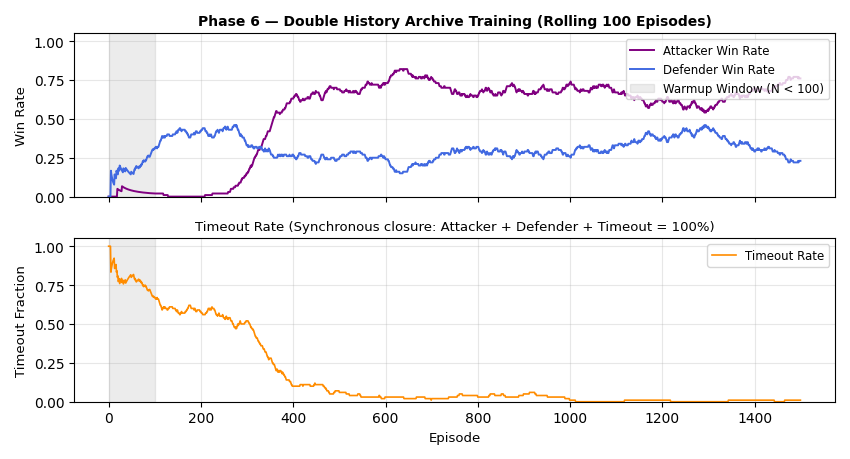
\includegraphics[width=0.92\columnwidth]{phase6_archive_curve.png}
\caption{Dual-Archive training over 1,500 episodes. Top: rolling win rates for the Attacker (purple, settling near $65\%$) and the Defender (blue, settling near $33\%$), which fits the structural advantage of three bridges against one defender. Bottom: the timeout rate falls from about $80\%$ during early exploration to below 2\% at convergence.}
\label{fig:training_curve}
\end{figure}

\section{Dual-Archive Co-Evolutionary Framework}

\subsection{Why Plain Self-Play Is Fragile}
Throughout the paper we call the three trained models by their phase in our experiments: Phase 3 is a fixed-opponent baseline, Phase 4 is direct self-play, and Phase 6 is the Dual-Archive model.

In direct self-play (Phase 4), the parameters $\theta_A$ and $\theta_D$ are updated against each other:
\begin{align}
\theta_{A, k+1} &\leftarrow \theta_{A, k} + \eta_A \nabla_{\theta_A} \mathcal{J}_A(\theta_{A, k}, \theta_{D, k}) \\
\theta_{D, k+1} &\leftarrow \theta_{D, k} + \eta_D \nabla_{\theta_D} \mathcal{J}_D(\theta_{A, k}, \theta_{D, k})
\end{align}
Because both updates happen at the same time, neither policy faces a fixed opponent. If the Attacker learns to break through the North bridge, the Defender adapts by guarding the North bridge. The Attacker then moves to the South bridge and may stop practicing North or Center. This can lead to cycling and to collapse onto a few routes.

\subsection{Dual-Archive Architecture}
To anchor learning without a large league-training system, we use a symmetric Dual-Archive method (Phase 6). We keep two reservoirs of past policies:
\begin{equation}
\mathcal{H}_A = \{\pi_A^{(1)}, \pi_A^{(2)}, \dots, \pi_A^{(K)}\}, \quad \mathcal{H}_D = \{\pi_D^{(1)}, \pi_D^{(2)}, \dots, \pi_D^{(K)}\}
\end{equation}
After a warm-up of $E_{\text{warm}} = 300$ episodes, a frozen copy of each active policy is added to its archive every $E_{\text{snap}} = 100$ episodes.

Each training episode uses one of three opponent settings:
\begin{itemize}
    \item \textbf{Active co-evolution (60\%):} The active Attacker plays the active Defender, and both update.
    \item \textbf{Attacker against history (20\%):} The active Attacker plays a Defender snapshot drawn uniformly, $\pi_D \sim \mathcal{U}(\mathcal{H}_D)$. Only the Attacker updates.
    \item \textbf{Defender against history (20\%):} The active Defender plays an Attacker snapshot drawn uniformly, $\pi_A \sim \mathcal{U}(\mathcal{H}_A)$. Only the Defender updates.
\end{itemize}
The 60\% share keeps both agents learning against current opponents, and the two 20\% shares expose each agent to older behavior, which is meant to limit forgetting.

\subsection{Actor-Critic PPO Implementation}
Both agents are trained with Proximal Policy Optimization (PPO) \cite{schulman2017proximal}. The actor $\pi_\theta(a \mid s)$ and critic $V_\phi(s)$ each have two fully connected layers of 64 units with $\tanh$ activations.

The policy is trained with the clipped surrogate objective
\begin{equation}
\mathcal{L}^{\text{CLIP}}(\theta) = \hat{\mathbb{E}}_t \left[ \min\left( r_t(\theta)\hat{A}_t, \, \text{clip}(r_t(\theta), 1-\epsilon, 1+\epsilon)\hat{A}_t \right) \right]
\end{equation}
where $r_t(\theta) = \frac{\pi_\theta(a_t \mid s_t)}{\pi_{\theta_{\text{old}}}(a_t \mid s_t)}$ and the clipping threshold is $\epsilon = 0.20$. Advantages are computed from discounted Monte Carlo returns, $\hat{A}_t = G_t - V_\phi(s_t)$, and standardized within each batch. Actions that would move into blocked cells are masked out.

Each update runs 4 epochs with minibatch size 64, and updates happen every 20 episodes (every 10 for the Phase 3 baseline). The total loss is
\begin{equation}
\mathcal{L}_{\text{total}}(\theta, \phi) = -\mathcal{L}^{\text{CLIP}}(\theta) + 0.5 \, \mathcal{L}^{\text{VF}}(\phi) - 0.01 \, \mathcal{S}[\pi_\theta](s_t)
\end{equation}
with learning rates $\alpha_{\text{actor}} = 10^{-3}$ and $\alpha_{\text{critic}} = 2 \times 10^{-3}$, and gradient-norm clipping at $\tau_{\text{clip}} = 0.5$.

\begin{figure*}[t]
\centering
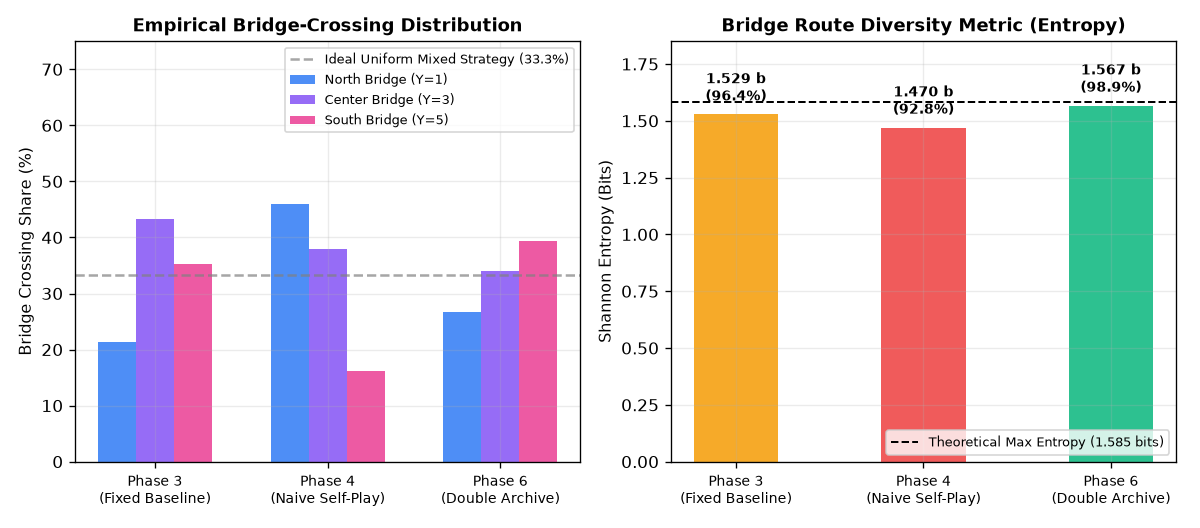
\includegraphics[width=0.90\textwidth]{bridge_diversity_chart.png}
\caption{Bridge-route diversity over 150 paired evaluation seeds. Left: share of crossings through the North ($Y=1$), Center ($Y=3$) and South ($Y=5$) bridges, with the uniform 33.3\% line for reference. Right: Shannon route entropy. Dual-Archive co-evolution (Phase 6) reaches 1.567 bits (98.9\% of the maximum), while direct self-play (Phase 4) shows an uneven route distribution and 17.3\% timeouts.}
\label{fig:bridge_diversity}
\end{figure*}

\section{Evaluation Methodology}

We use two evaluation protocols to compare route use and exploitability.

\subsection{Route Diversity via Shannon Entropy}
We record successful river crossings at $X=5$ over 150 paired evaluation seeds. The Attacker plays against a passive Defender that stays in place, so route choice is measured without active interception. A crossing counts when the Attacker reaches $X \ge 6$. This shows which routes the policy uses; it does not show whether the policy could still use a route it rarely picks.

Let $C_b$ be the number of successful crossings through bridge $b \in \{b_N, b_C, b_S\}$. The share of crossings through each bridge is
\begin{equation}
p_b = \frac{C_b}{\sum_{k \in \{N, C, S\}} C_k}
\end{equation}
and the Shannon route entropy is
\begin{equation}
H(\text{Routes}) = -\sum_{b \in \{N, C, S\}} p_b \log_2(p_b)
\end{equation}
Its bounds are
\begin{align}
H_{\max} &= \log_2(3) \approx 1.585 \text{ bits} \quad (\text{uniform, 33.3\% per route}) \\
H_{\min} &= 0 \text{ bits} \quad (\text{all crossings on one bridge})
\end{align}
The diversity ratio is $\rho_{\text{div}} = \frac{H(\text{Routes})}{H_{\max}} \times 100\%$. A timeout is an episode in which the Attacker does not cross within 75 steps.

\subsection{Empirical Game-Theoretic Analysis (EGTA)}
To judge how close a policy is to a minimax solution without relying only on win rates, we use an empirical game-theoretic analysis. We build a suite of defenders $\mathcal{P}_{\text{def}}$:
\begin{enumerate}
    \item \textbf{North Camper ($Y=1$):} A static blocker parked at the North bridge.
    \item \textbf{Center Camper ($Y=3$):} A static blocker at the Center bridge.
    \item \textbf{South Camper ($Y=5$):} A static blocker at the South bridge.
    \item \textbf{River Patroller:} A defender that sweeps back and forth along the east bank of the river between $Y=1$ and $Y=5$.
    \item \textbf{Learned Defenders:} The trained neural policies $\pi_{D, \text{Phase 4}}$ and $\pi_{D, \text{Phase 6}}$.
\end{enumerate}

The empirical payoff matrix $\bm{M} \in \mathbb{R}^{m \times n}$ holds the Attacker's net win margin of Attacker policy $i$ against defender $j$:
\begin{equation}
M_{i, j} = \text{WinRate}(\pi_i, d_j) - \text{CatchRate}(\pi_i, d_j) \in [-1.0, +1.0]
\end{equation}
From $\bm{M}$ we compute:
\begin{enumerate}
    \item \textbf{Minimax game value ($v^*$):} Found with 50,000 iterations of zero-sum Fictitious Play on the empirical meta-game, giving $v^* = -0.046$.
    \item \textbf{Security level ($v_{\text{sec}}$):} The worst net margin of policy $\pi_i$ against any defender in the suite:
    \begin{equation}
    v_{\text{sec}}(\pi_i) = \min_{j \in \mathcal{P}_{\text{def}}} M_{i, j}
    \end{equation}
    \item \textbf{Empirical exploitability ($\delta_{\text{meta}}$):} The gap between the game value and the security level:
    \begin{equation}
    \delta_{\text{meta}}(\pi_i) = v^* - v_{\text{sec}}(\pi_i)
    \end{equation}
\end{enumerate}
A lower $\delta_{\text{meta}}$ means the policy is closer to the minimax value within the set of strategies we tested.

\section{Results and Discussion}

\begin{table*}[t]
\caption{Bridge Crossing Distribution and Route Diversity ($N=150$ Paired Evaluation Seeds)}
\label{tab:bridge_diversity}
\centering
\begin{tabular}{lccccccc}
\toprule
\textbf{Model} & \textbf{North ($Y=1$)} & \textbf{Center ($Y=3$)} & \textbf{South ($Y=5$)} & \textbf{Timeouts} & \textbf{Entropy ($H$)} & \textbf{Diversity \%} & \textbf{Profile} \\
\midrule
Phase 3 (Fixed Baseline)        & 21.3\% & 43.3\% & 35.3\% & 0.0\%  & 1.529 bits & 96.4\% & Baseline navigation \\
Phase 4 (Direct Self-Play)      & 46.0\% & 37.9\% & 16.1\% & 17.3\% & 1.470 bits & 92.8\% & North-heavy, 17.3\% timeouts \\
\textbf{Phase 6 (Dual Archive)} & \textbf{26.7\%} & \textbf{34.0\%} & \textbf{39.3\%} & \textbf{0.0\%}  & \textbf{1.567 bits} & \textbf{98.9\%} & \textbf{Balanced use of all three bridges} \\
\bottomrule
\end{tabular}
\end{table*}

\begin{table*}[t]
\caption{Meta-Game Security Levels and Exploitability ($N=150$ Paired Evaluation Seeds)}
\label{tab:exploitability}
\centering
\begin{tabular}{lccccc}
\toprule
\textbf{Attacker Policy} & \textbf{Security Level ($v_{\text{sec}}$)} & \textbf{Worst-Case Win Rate} & \textbf{Exploitability ($\delta$)} & \textbf{Average Win Margin} & \textbf{Patroller Win Rate} \\
\midrule
Phase 4 (Direct Self-Play)      & -0.207 & 39.3\% & 0.160 & +0.190 & 76.0\% \\
\textbf{Phase 6 (Dual Archive)} & \textbf{-0.187} & \textbf{31.3\%} & \textbf{0.140} & \textbf{+0.184} & \textbf{81.3\%} \\
\bottomrule
\end{tabular}
\end{table*}

\subsection{Route Use Under Archive Training}
Table~\ref{tab:bridge_diversity} and Fig.~\ref{fig:bridge_diversity} show the crossing distributions.

The direct self-play agent (Phase 4) favors one side. It sends 46.0\% of its crossings through the North bridge and only 16.1\% through the South bridge, and its entropy is 1.470 bits (92.8\% of the maximum). It also times out in 17.3\% of episodes even though the river is undefended. A likely explanation is that when the spawn point makes the North bridge hard to reach, the policy does not redirect to the southern bridges and runs out of time. We have not tested this explanation directly.

The Dual-Archive policy (Phase 6) spreads its crossings over all three bridges: 26.7\% North, 34.0\% Center, and 39.3\% South. Its entropy is \textbf{1.567 bits}, or \textbf{98.9\% of the maximum} (1.585 bits), and it has \textbf{no timeouts}. A plausible reason is that it trained against archived defenders that had guarded different bridges, so it kept using several routes. Our measurements show this pattern but do not prove the cause.

\begin{figure*}[!t]
\centering
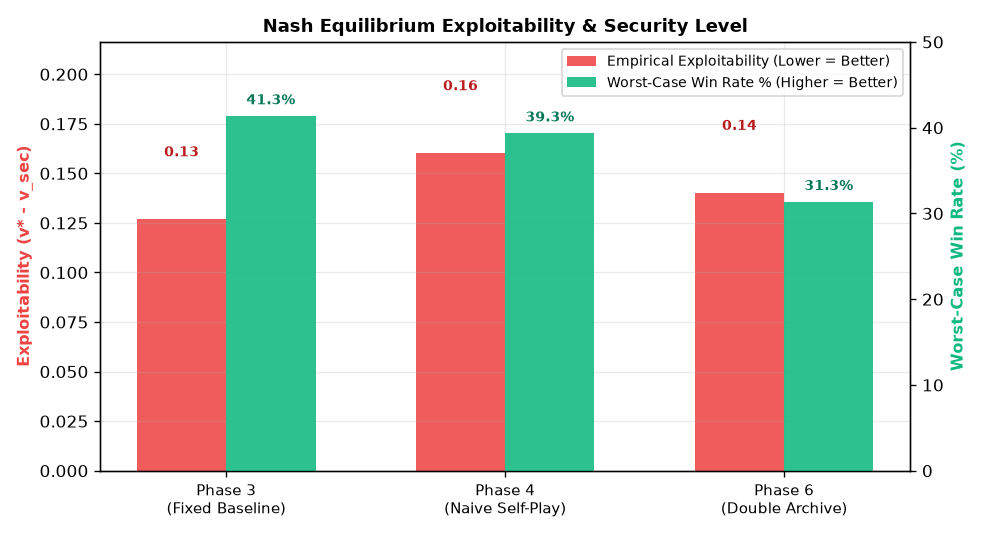
\includegraphics[width=0.78\textwidth]{nash_exploitability_chart.png}
\caption{Empirical exploitability ($\delta$) and worst-case win rate against the tested defender types. Dual-Archive co-evolution lowers exploitability from 0.160 to 0.140 and raises the security level from $-0.207$ to $-0.187$.}
\label{fig:nash_exploitability}
\end{figure*}

\subsection{Exploitability}
Table~\ref{tab:exploitability} and Fig.~\ref{fig:nash_exploitability} give the meta-game results.

Dual-Archive training lowers empirical exploitability $\delta_{\text{meta}}$ from $0.160$ to \textbf{0.140}, a 12.5\% reduction, and raises the security level from $-0.207$ to \textbf{$-0.187$}. Against the River Patroller, the Phase 6 win rate rises from 76.0\% to 81.3\%.

The Attacker's worst-case win rate in the defender pool is 31.3\% for Phase 6 and 39.3\% for Phase 4. In both cases the worst result comes against the Phase 6 Defender. This is consistent with the Phase 6 Defender also having trained against archived attackers, which may have taught it better lateral interception, so that even a more varied Attacker has trouble against it.

Pooled over all 150 paired seeds per defender, the win-rate difference between Phase 6 and Phase 4 is $\Delta = -0.6\%$ (95\% CI: $-4.3\%$ to $+3.2\%$; $z = -0.29$, $p = 0.771$). This is not statistically significant. Route entropy and exploitability give extra views of the two policies, but neither one shows that a policy holds up against every possible opponent.

\subsection{Training Dynamics and Reward Shaping}
Fig.~\ref{fig:training_curve} shows Phase 6 training over 1,500 episodes. During the 300 warm-up episodes, the timeout rate stays high ($\approx 80\%$) while the agents learn basic navigation. Once archive sampling starts at episode 300, the timeout rate falls below 2\%, and the rolling win rates settle near $65\%$ for the Attacker and $33\%$ for the Defender. This split matches the layout of the arena: an Attacker with the same speed as the Defender has three crossings to choose from against a single defender.

We also checked step rewards across environment transitions. In every transition, $R_A + R_D = 0$ held to machine precision. Using the same discount $\gamma = 0.99$ in \eqref{eq:shaping_tgt}, \eqref{eq:shaping_rel} and the PPO value network matches the conditions of Ng et al. \cite{ng1999policy}.

\section{Multi-Target Extension: Dual-Flank Perimeter Arena ($K=2$)}
\label{sec:multi_target}

We ran a separate experiment in which the Attacker can choose between several targets. These results use 500 episodes and are separate from the 150 paired seeds in the main evaluation.

\subsection{Multi-Target Formulation}
Here the Attacker wins by reaching any one of $K \ge 2$ target cells $\{T_0, T_1, \dots, T_{K-1}\}$ instead of a single Citadel. In the main $K=2$ setup, two targets sit on the east edge in line with the North and South bridges: $T_0 = (10, 1)$ and $T_1 = (10, 5)$.

So that one network design can handle different target counts, the observation is expanded to a normalized 19-dimensional vector:
\begin{equation}
s_t = \left[ \tilde{x}_A, \tilde{y}_A, \tilde{x}_D, \tilde{y}_D, \tilde{x}_{T_0}, \tilde{y}_{T_0}, a_0, \dots, \tilde{x}_{T_4}, \tilde{y}_{T_4}, a_4 \right]^T
\end{equation}
where $\tilde{x} = x / (W-1)$, $\tilde{y} = y / (H-1)$, and $a_k \in \{0, 1\}$ marks whether target $k$ is active (unused slots with $k \ge K$ are padded with inactive entries).

To keep the shaping policy-invariant with $\gamma = 0.99$ (Ng et al. \cite{ng1999policy}), the potential is the distance to the nearest active target:
\begin{equation}
\Phi_{\text{multi}}(s) = \min_{k \in \{0, \dots, K-1\}} D(s_A, T_k)
\end{equation}
where $D(s_A, T_k)$ is the obstacle-aware distance that goes through a valid bridge. The shaping reward is
\begin{equation}
F_{\text{target}}(s, s') = \left( \min_{k} D(s_A, T_k) - \gamma \min_{k} D(s'_A, T_k) \right) \cdot \alpha_{\text{target}}
\end{equation}
As before, we set $R_A^{\text{shaping}} = +F_{\text{target}} - F_{\text{rel}}$ and $R_D^{\text{shaping}} = -F_{\text{target}} + F_{\text{rel}}$, so the rewards still sum to zero in every multi-target episode.

\subsection{Effect of the Number of Targets ($K \in \{1, 2, 3, 5\}$)}
We evaluated each target setting over 500 episodes with a 100-step horizon. $K=1$ uses the central target, $K=2$ the north and south targets, $K=3$ the three bridge-aligned targets, and $K=5$ five open cells on the east edge. Table~\ref{tab:attacker_k_scaling} gives Attacker win rates, and Table~\ref{tab:defender_k_scaling} gives Defender capture rates for the same defender types and target counts.

\begin{table}[t]
\caption{Attacker Win Rate (\%) by Target Count ($K \in \{1,2,3,5\}$, $N=500$, $T=100$)}
\label{tab:attacker_k_scaling}
\centering
\resizebox{\columnwidth}{!}{%
\begin{tabular}{lcccc}
\toprule
\textbf{Defender Type} & \textbf{$K=1$} & \textbf{$K=2$} & \textbf{$K=3$} & \textbf{$K=5$} \\
\midrule
Learned Defender & 15.2\% & 68.4\% & 97.6\% & 89.2\% \\
Center Camper ($Y=3$) & 0.0\% & 74.4\% & 70.4\% & 69.4\% \\
North Camper ($Y=1$) & 14.0\% & 74.2\% & 62.6\% & 60.6\% \\
South Camper ($Y=5$) & 13.8\% & 52.6\% & 68.2\% & 71.2\% \\
River Patroller & 9.4\% & 83.2\% & 86.2\% & 86.2\% \\
Stationary Stay & 12.2\% & 85.0\% & 82.6\% & 82.6\% \\
Greedy Pursuit & 5.8\% & 34.4\% & 28.2\% & 30.8\% \\
Random Walk & 22.4\% & 84.6\% & 84.8\% & 87.2\% \\
\bottomrule
\end{tabular}%
}
\end{table}

\begin{table}[t]
\caption{Defender Capture Rate (\%) by Target Count ($K \in \{1,2,3,5\}$, $N=500$, $T=100$)}
\label{tab:defender_k_scaling}
\centering
\resizebox{\columnwidth}{!}{%
\begin{tabular}{lcccc}
\toprule
\textbf{Defender Type} & \textbf{$K=1$} & \textbf{$K=2$} & \textbf{$K=3$} & \textbf{$K=5$} \\
\midrule
Learned Defender & 7.4\% & 31.6\% & 2.4\% & 10.8\% \\
Center Camper ($Y=3$) & 14.0\% & 25.6\% & 29.6\% & 30.6\% \\
North Camper ($Y=1$) & 25.8\% & 25.8\% & 37.4\% & 39.4\% \\
South Camper ($Y=5$) & 16.0\% & 47.4\% & 31.8\% & 28.8\% \\
River Patroller & 8.4\% & 16.8\% & 13.8\% & 13.8\% \\
Stationary Stay & 7.8\% & 15.0\% & 17.4\% & 17.4\% \\
Greedy Pursuit & 59.4\% & 65.6\% & 71.8\% & 69.2\% \\
Random Walk & 31.2\% & 15.4\% & 15.2\% & 12.8\% \\
\bottomrule
\end{tabular}%
}
\end{table}

The tables report Attacker wins and Defender captures. These are separate terminal outcomes; the timeout percentage for each matchup is the remainder after subtracting both from 100\%. In the configurable $K=1$ benchmark against the learned Defender, for example, 15.2\% were Attacker wins, 7.4\% were captures, and 77.4\% timed out. This result differs from the original six-input Citadel baseline because the policies and training setup differ.

\begin{figure*}[!t]
\centering
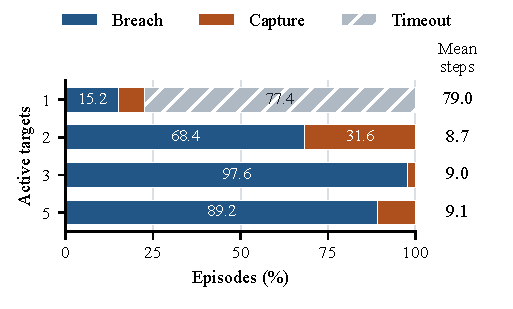
\includegraphics[width=0.78\textwidth]{paper_figures/multi_target_outcomes_and_duration.pdf}
\caption{Attacker wins, Defender captures, timeouts, and mean episode length against the learned Defender across target counts. Each layout uses 500 evaluation episodes.}
\label{fig:scaling_diagnostics}
\end{figure*}

The two tables report the Attacker win and Defender capture rates for each defender type. Fig.~\ref{fig:scaling_diagnostics} also shows timeouts and episode length for the learned Defender. Its Attacker win rate rises from $15.2\%$ at $K=1$ to $97.6\%$ at $K=3$, then falls to $89.2\%$ at $K=5$, so the trend is not monotonic. We did not test why $K=5$ is lower than $K=3$.

\subsection{Route Use in the $K=2$ Evaluation}
In the same 500-episode evaluation, the Attacker reached a target in 342 episodes. Of these, 128 (37.4\%) were at the North target and 214 (62.6\%) at the South target. The recorded bridge crossings were 131 North, 128 Center, and 241 South. These counts describe this run only and do not show that the policy would use both targets equally against other opponents.

Fig.~\ref{fig:target_choices} compares bridge entries with successful target breaches across all four layouts. Bridge entries can include episodes that later end in a capture or timeout, while a breach count includes only episodes in which the Attacker reaches a target.
\begin{figure*}[!t]
\centering
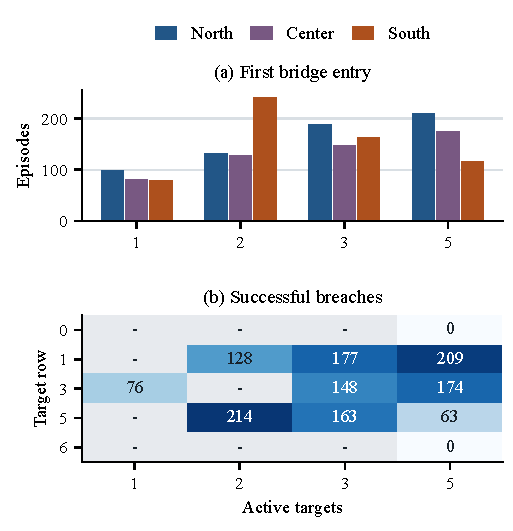
\includegraphics[width=0.78\textwidth]{paper_figures/multi_target_bridge_and_breach_counts.pdf}
\caption{First bridge entries and successful target breaches against the learned Defender. Entry counts include episodes that later ended in capture or timeout; breach counts include Attacker wins only.}
\label{fig:target_choices}
\end{figure*}

A separate training audit found that the timeout rate fell from 34.0\% during warm-up to 0.00\% by episode 300. Across 11 saved policy snapshots, the Attacker won 69\% of episodes and the Defender caught it in 30\%. This audit is separate from the 500-episode evaluation behind Tables~\ref{tab:attacker_k_scaling} and~\ref{tab:defender_k_scaling}.

\section{Limitations and Future Work}
Several points limit how far these results can be taken:
\begin{enumerate}
    \item \textbf{Single training run:} The single-target comparisons use 150 paired evaluation seeds per matchup, and the multi-target section uses 500 episodes. All results come from one representative training run per method. Repeating training with several random seeds would show how much the results vary between runs.
    \item \textbf{No direct test of forgetting:} We measure route use and exploitability. We do not test whether an agent loses the ability to use a route, so the link to catastrophic forgetting is only suggested.
    \item \textbf{Archive sampling:} We sample uniformly from the archive, $\mathcal{U}(\mathcal{H})$. In longer training runs this may spend updates on obsolete early policies. Prioritized fictitious play or regret-weighted sampling would be a natural next step.
    \item \textbf{Continuous action spaces:} Moving from discrete grid bottlenecks to continuous navigation would call for ways to compress or cluster the archive.
\end{enumerate}

\section{Conclusion}
We compared direct self-play with Dual-Archive Co-Evolution in the Three Bridges Arena. In the main evaluation, direct self-play favored the North bridge (46.0\% of crossings) over the South bridge (16.1\%), and 17.3\% of its episodes timed out. The archive-trained policy had higher route entropy and no timeouts. Its exploitability was lower (0.140 versus 0.160) and its security score was higher ($-0.187$ versus $-0.207$), although the pooled win-rate difference was not statistically significant. These results suggest that archive training may help keep route use varied in this setting. The study does not measure catastrophic forgetting directly, and the findings should be checked with more independent training runs and more opponents.

\appendices
\section{Simplified Three-Route Matching Model}
\label{app:matching}
This appendix analyzes a deliberately small model with three Attacker route choices and three Defender guard choices. The Defender's payoff is $+1$ when it guards the route chosen by the Attacker and $-1$ otherwise. With Attacker routes as rows and Defender choices as columns, the payoff matrix is
\begin{equation}
M_D = \begin{bmatrix} +1 & -1 & -1 \\ -1 & +1 & -1 \\ -1 & -1 & +1 \end{bmatrix}.
\end{equation}
There is no pure-strategy equilibrium: when the choices match, the Attacker can switch to an unguarded route; when they differ, the Defender can switch to the Attacker's route. If both players choose uniformly, the Defender's expected payoff against any pure action of the opponent is
\begin{equation}
\mathbb{E}[M_D] = \frac{1}{3}(+1)+\frac{2}{3}(-1)=-\frac{1}{3}.
\end{equation}
The uniform mixtures are minimax strategies for this matching matrix. This result illustrates the value of mixing in the simplified model; it does not establish an equilibrium for the full grid game.

\section*{Acknowledgment}
The authors thank the Department of Mathematics at Sardar Vallabhbhai National Institute of Technology (SVNIT), Surat, for providing computational facilities and academic guidance throughout this work.

\begin{thebibliography}{3}
\bibitem{cliff1995tracking} D. Cliff and G. F. Miller, ``Tracking the Red Queen: Measurements of adaptive progress in co-evolutionary simulations,'' in \textit{Proc. Eur. Conf. Artif. Life (ECAL)}, 1995, pp. 200--218.
\bibitem{ng1999policy} A. Y. Ng, D. Harada, and S. Russell, ``Policy invariance under reward transformations: Theory and application to reward shaping,'' in \textit{Proc. Int. Conf. Mach. Learn. (ICML)}, 1999, pp. 278--287.
\bibitem{schulman2017proximal} J. Schulman, F. Wolski, P. Dhariwal, A. Radford, and O. Klimov, ``Proximal policy optimization algorithms,'' \textit{arXiv preprint arXiv:1707.06347}, 2017.
\end{thebibliography}

\end{document}
